\section{Testing}
In der Python Standard Library gibt es das Unit Testing Framework \textbf{unittest}, das es erlaubt Unittests zu implementieren. 
Django's Unit tests basieren auf dieser Library und erweitern diese, beispielsweise erbt \textbf{django.test.TestCase} von \textbf{unittest.TestCase}. Weiter werden auch Integrationtests ermöglicht.

\subsubsection{Beispiel Integrationtests}
\begin{python}
from django.test import Client, TestCase
from django.contrib.auth.models import User

class AboutViewsTests(TestCase):

   def setUp(self):
       self.user = User.objects.create(username='testuser')
       self.user.set_password('12345')
       self.user.save()
       self.client = Client()
       self.client.login(username='testuser', password='12345')

   def test_about_get(self):
       response = self.client.get('/about/')
       self.assertEquals(response.status_code, 200)      
\end{python}

\subsection{Continuous Integration (CI)}
\subsubsection{Anforderungen}
\begin{itemize}
	\item Aufbau von IPsec Tunnel zwischen mindesten zwei Rechnern
	\item automatisierter Ablauf
	\item geringe Einarbeitungszeit in Technologien
	\item möglichst kostenfreie Dienste nutzen
\end{itemize}
\subsubsection{Tools}
\paragraph{GitHub} wird von uns als online Repository verwendet und wird mit dem Versionsverwaltungssystem Git eingesetzt. Weiter bietet es für andere Dienste WebHooks an. 
\paragraph{Travis CI} wird als eigentlicher Continuous Integration Anbieter verwendet, es werden automatisierte Builds und Tests ermöglicht. Travis CI ist für Projekte, welche auf GitHub gehostet werden ausgelegt.

\paragraph{Docker} um Integration Tests zu ermöglichen wird docker-compose eingesetzt, welches gewährleistet mehrere Docker Container zu builden und eine Netzwerk untereinander aufzubauen. \\
\decision{Toolstack CI}
Um einen IPsec Tunnel aufzubauen nutzen wir zwei Docker Container mit Hilfe von docker-compose. Travis CI unterstützt docker-compose und lässt sich nahtlos mit GitHub kombinieren. Diese Technologien sind uns schon bekannt und werden kostenlos zur Verfügung gestellt.

\begin{figure}[H]
\centering
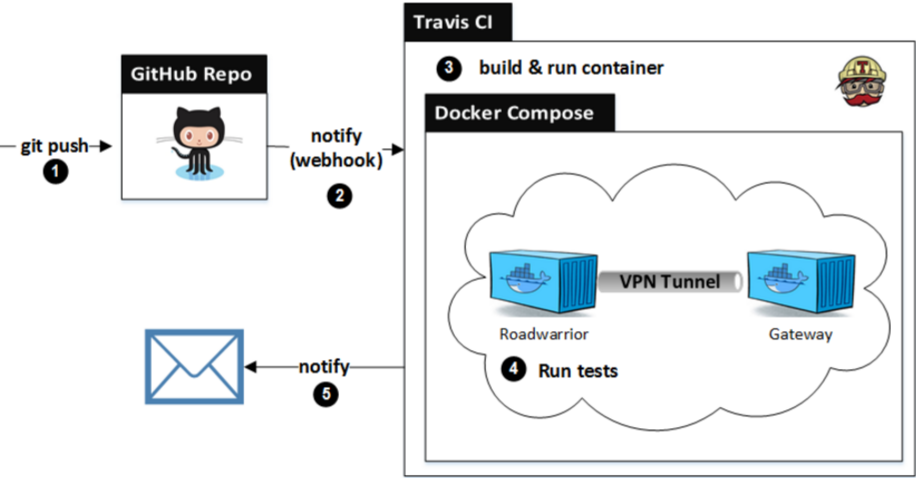
\includegraphics[width=420pt]{images/testing.png}
\caption[Schematische Darstellung der Testumgebung]{Schematische Darstellung der Testumgebung}
\end{figure}
\subsubsection{Ablauf}
\begin{enumerate}
	\item git push, lokaler Code wird auf GitHub publiziert
	\item Travis CI wird durch WebHook notifiziert
	\item Travis CI buildet zwei Docker Container, welche auf der Basis des offiziellen Django Container aufbauen 
	\begin{enumerate}
         \item StrongSwan mit den nötigen Plugins wird installiert und gestartet
         \item Auf dem Roadwarrior wird die strongMan Applikation vom GitHub Repository installiert und der aktuelle Branch wird eingecheckt
      \end{enumerate}
      \item Der Roadwarrior started die Unit- sowie die Integrationstests, dabei werden zwischen den Docker Container diverse Ipsec Tunnels auf- und abgebaut
      \item abschliessend wird über Erfolg oder Misserfolge per Email notifiziert
\end{enumerate}
